Why do I have a blank first page in this?


\documentclass[review,jog]{igs}
% \documentclass[review,aog]{igs}

\usepackage[utf8]{inputenc}

\usepackage{mathabx}
\usepackage{graphicx}
\usepackage{siunitx}

% the default is for unnumbered section heads
% if you really must have numbered sections, remove
% the % from the beginning of the following command
% and insert the level of sections you wish to be
% numbered (up to 4):

\setcounter{secnumdepth}{2 }

\jourvolume{X}
\jourissue{X}
\jourpubyear{2025}

\begin{document}

\title[Modelling recurring Jökulhlaup in 2D]{A physical representation of recurring Jökulhlaup floods in a fully-coupled subglacial hydrology model}.


\author[Hepburn and others]{Adam J. HEPBURN,$^{1,*}$
Sammie BUZZARD,$^{2}$
Stephen LIVINGSTONE,$^{3}$
Samuel DOYLE,$^{1,3}$
Rob STORRAR,$^{4}$
Laura EDWARDS,$^{5}$
Andrew SOLE,$^{3}$
Ryan ING,$^{6}$
Neil ROSS,$^{7}$
Liz BAGSHAW,$^{8}$
Matthew PEACEY,$^{1,8}$
Thomas CHUDLEY,$^{9}$
Caroline CLASON,$^{9}$
Michael PRIOR-JONES,$^{10}$
Gialuca BIANCHI,$^{10}$
Jonathon HAWKINGS,$^{10}$
Tifen LE BRIS,$^{11}$
Guilhem BARRUOL,$^{11}$
Florent GIMBERT,$^{11}$
Adrien GILBERT,$^{11}$
Alexandre MICHEL,$^{11}$
Christine DOW,$^{12}$
Tun Jan YOUNG,$^{13}$
Sian THORPE,$^{3}$
Adam BOOTH,$^{14}$
Lisa CRAW,$^{10}$
Angus MOFFATT,$^{3}$
Remy VENESS,$^{4}$
Siobhan KILLINGBECK,$^{15}$
Sarah MANN,$^{10}$
Andrew JONES,$^{4}$  
}

\affiliation{%
$^1$Centre for Glaciology, Department of Geography and
  Earth Sciences, Aberystwyth University, Aberystwyth,
  UK\\
  $^2$Northumbria University, UK, \\
$^3$The University of Sheffield, UK, \\
$^4$Sheffield Hallam University, UK, \\
$^5$Liverpool John Moores University, UK, \\
$^6$University of Edinburgh, UK, \\
$^7$Newcastle University, UK, \\
$^8$University of Bristol, UK, \\
$^9$Durham University, UK, \\
$^{10}$Cardiff University, UK, \\
$^{11}$Université de Grenoble/CNRS, France, \\
$^{12}$University of Waterloo, Canada, \\
$^{13}$St. Andrews University, UK, \\
$^{14}$University of Leeds, UK, \\
$^{15}$Swansea University, UK,

  $^{*}$Correspondence: Adam J. Hepburn 
  \email{adam.hepburn@aber.ac.uk}}

\begin{frontmatter}

\maketitle

\begin{abstract}
Abstract stuff
\end{abstract}

\end{frontmatter}


\section{Introduction}

\section{Method}



The work presented here is an extension to the Glacier Drainage System (GlaDS) model \citep{werder2013modeling}, building upon earlier 1-dimensional work \citep{kingslake2013modelling} in order to incorporate a physically-consistent representation of ice-marginal lake drainage in 2 dimensions. Our work includes multiple couplings between the subglacial hydrological system and the ice-marginal lake, as well as between each of these and ice-velocity (Fig.~\ref{FIG:1}). In Section~\ref{methods:GlaDS} we describe the GlaDS model and relevant modifications to the version originally presented by \citep{werder2013modeling}. In Section~\ref{methods:Lake} we describe the lake-drainage equations. In Section~\ref{methods:coupling} we describe the coupling between hydrology and ice-dynamics, and our method of numerical solution is presented in Section~\ref{methods:Numeric}. 

\begin{figure}
\centering{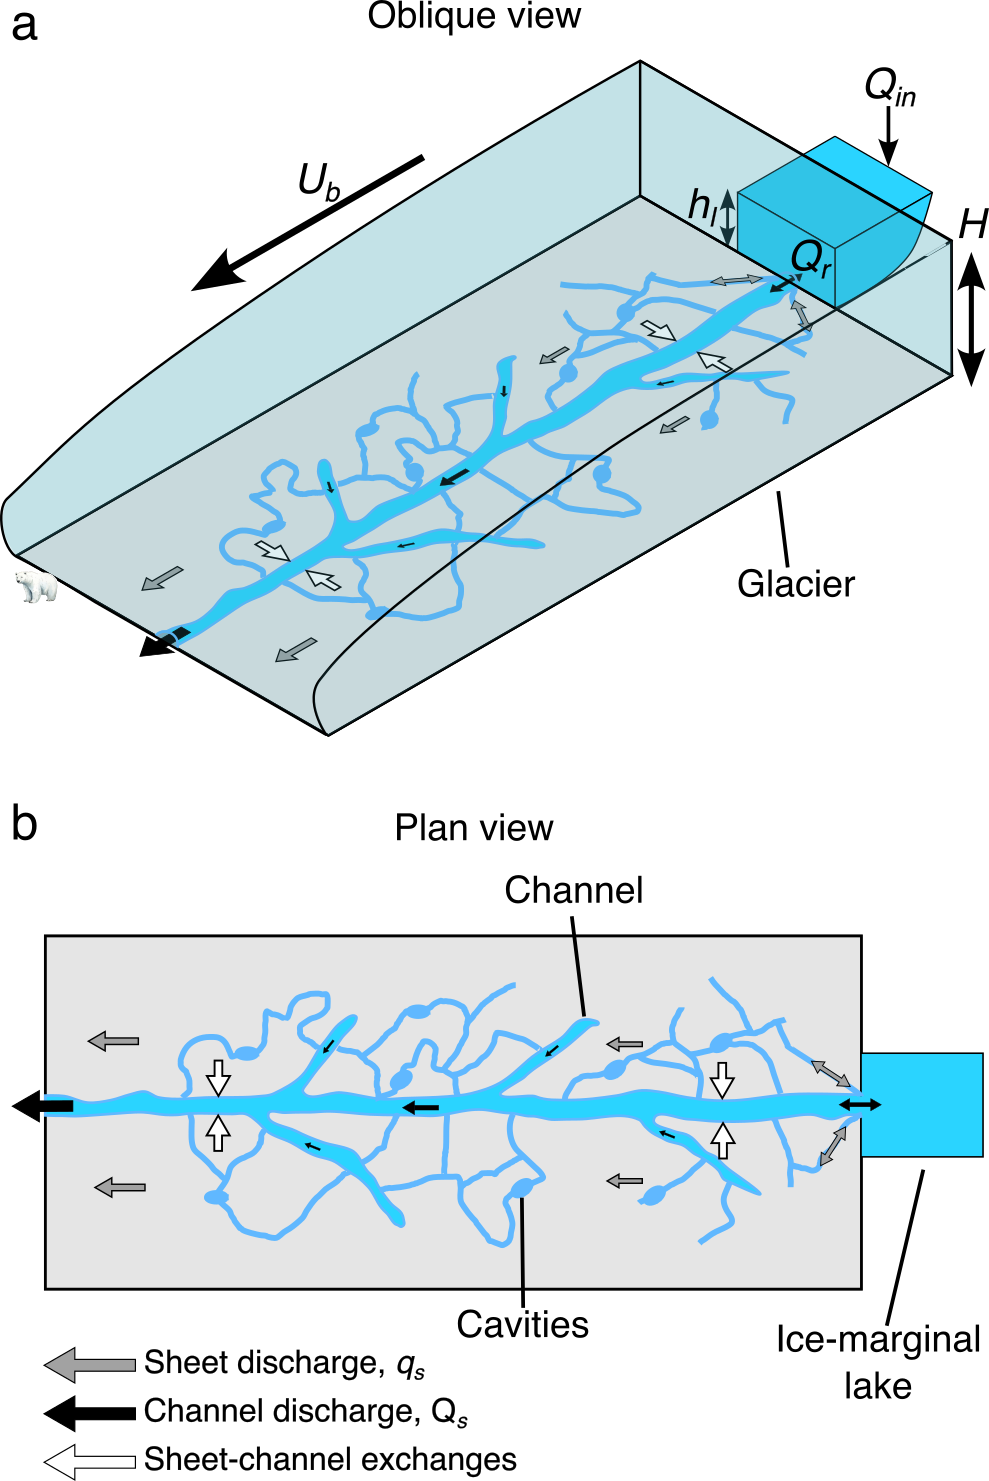
\includegraphics{./figures/Figure_1/Figure1.png}}
\caption{Schematic illustration of our model. \textbf{a}) Oblique view showing an ice-marginal lake connected two-ways to a subglacial channel and sheet. This in turn modifies basal velocity, $U_{b}$ through effective pressure, $N$. \textbf{b}) plan view of the same system. Note, although the ice-marginal lake is shown as connected to one channel, in our model an ice-marginal lake can be connected to the subglacial system at multiple outlets. \texttt{[SINGLE-COLUMN]}}
\label{FIG:1}
\end{figure}

\begin{figure*}
\centering{\includegraphics[width=1\textwidth]{./figures/Figure_3/Figure3.png}}
\caption{Caption continue overleaf. }
\label{FIG:3}
\end{figure*}
\clearpage
\addtocounter{figure}{-1}
\noindent\captionof{figure}{Evolution of the 'baseline' model configuration in our synthetic modelling domain. \textbf{a}) Lake height, $l_{h}$ through time. Black points indicate $l_{h}$ in panels \textbf{c}--\textbf{e}. \textbf{b}) Sum discharge at the lake outlet, $Q_{r}$ through time. Grey points indicate $Q_{r}$ in panels \textbf{c}--\textbf{e} the grey box indicates the time span of panel \textbf{g}. \textbf{c}--\textbf{e}) Channel discharge, $Q_{c}$ at $t=$7.10 years (\textbf{c}), 8.38 years (\textbf{d}) and 9.00 years (\textbf{e}). In each panel, effective pressure, $N$ is shown as grey contours. \textbf{f}) Phase-plane diagram showing the evolution of $Q_{r}$ and $N$ through time at the ice-marginal lake outlet. Arrows and shading indicate the direction of time. The horizontal dashed line denotes the lake refill rate, $Q_{in} \equals$ 10 m$^{3}$s$^{-1}$. The vertical dashed line indicates $N$ when $l_{h}=$0 m. \textbf{g}) Filled contour plot showing the across-flow averaged velocity through time. White contours represent velocity (every 10 ma$^{-1}$) and the black line shows $Q_{r}$ between years 7--9.}

\begin{figure*}
\centering{\includegraphics[width=1\textwidth]{./figures/Figure_4/Figure4.png}}
\caption{\textbf{NOT FINAL VERSION!} Lake height, $l_{h}$ (left panels, i) and sum discharge at the lake outlet, $Q_{r}$ (right panels, ii) across a range of key model parameters. \textbf{a}) Channel conductivity, $k_c$. \textbf{b}) Sheet conductivity, $k_s$. \textbf{c}) Basal bump height, $h_{b}$. \textbf{d}) Channel sheet width, $l_c$.\textbf{e}) Cavity spacing, $l_{r}$. \textbf{f}) Basal melt rate, $M_r$. \textbf{g}) Lake refill rate, $Q_{in}$. In all panels, the default parameter run is shown in grey.}
\label{FIG:4}
\end{figure*}


\subsection{Subglacial Drainage}\label{methods:GlaDS}

The GlaDS model itself is a widely implemented (REF) 2D representation of subglacial hydrology. Operating on the an anisotropic mesh generated using ISSM, GlaDS includes a description of i) distributed flow through a series of linked cavities represented as a continuous sheet with variable thickness, and ii) channelised flow through Röthlisberger channels that are represented along element edges. Sheet elements exchange water with channels, and the cross-sectional area of these channels evolves through time due to the dissipation of potential energy, sensible heat exchange, and cavity closure rates due to viscous ice creep. Flux in both the distributed and channelised systems is driven by gradients in hydraulic potential, $\Delta \phi$. We refer interested readers to Appendix~\ref{Appendix:GlaDS} for an overview of key GlaDS equations, and to \cite{werder2013modeling} for a full descriptions of the equations governing water flow in GlaDS.

We note two key differences between the original GlaDS and the version described here: i) rather than assuming water flow within the sheet to always be turbulent \citep[cf:][]{werder2013modeling}, we make use of the \cite{hill2024improved} transition parametrisation, whereby sheet flow switches between laminar and turbulent flow according to the local Reynolds number, and ii) following \cite{Stevens2022}, we implement a viscously deforming 'elastic layer' which crudely represents hydraulic jacking where water pressure exceeds ice overburden pressure (SUPP EQ). 

\subsection{Lake evolution}\label{methods:Lake}

Following \cite{kingslake2013modelling} lake depth, $h_{l}$ (Fig.~\ref{fig:Schematic}), evolves with the continuity equation:

\begin{equation}
\label{eq:lakecontinuity}
\begin{aligned}
\frac{\delta h_{l}}{\delta t} = \frac{1}{A_{L}}[Q_{in}-Q{r}(t-1)],
\end{aligned}
\end{equation}
\noindent
where $A_L$ is the uniform lake area, $Q_{in}$ represents extraglacial lake input (e.g., rainfall, surface runoff) and $Q_{r}$ represents inflow/outflow at the lake outlet(s) from the previous timestep. In moving from a 1D to 2D representation of subglacial hydrology and including the contribution from the sheet, $Q_{r}$ in our model is given by:

\begin{equation}
\label{eq:sumQr}
\begin{aligned}
Q_{r}(t) = \sum_{i=1}^{N} \left( q_{s,i}(t) + Q_{c,i}(t) \right),
\end{aligned}
\end{equation}
\noindent
or the sum of the width integrated sheet discharge, $q_{s}$, and channel discharge, $Q_{c}$ along $N$ vertices connected to an ice-marginal lake. Following Eqn(~\ref{appeq:GlaDSdirBC}), hydrostatic lake pressure fixes the lake outlet hydraulic potential, $\phi_{outlet}$ to be: 

\begin{equation}
\label{eq:lakephi}
\begin{aligned}
\phi_{outlet} (t) = \rho_{w}gz_{b} + \rho_{w}gh_{l}(t) ,
\end{aligned}
\end{equation}

at all times, coupling an ice-marginal lake to the subglacial hydrological system through an additional Dirichlet boundary condition in GlaDS. 

\subsection{Friction and ice flow}\label{methods:coupling}

To couple ice-flow to hydrology in our synthetic domain (Section~\ref{application:synth}) we use a Budd style friction law of the form:






in our synthetic domain,
In our Greenland domain (Section~\ref{application:greenland}), with observational constraint on surface velocity, we use a Schoof-type friction law \citep{schoof2005effect} of the form: 

\begin{equation}
\label{eq:Schoof}
\begin{aligned}
\tau_b=\frac{C_s^2 v_b^m}{\left(1+\left(\frac{C_s^2}{C_{\max } N}\right)^{1 / m} u_b\right)^m},
\end{aligned}
\end{equation}

where $tau_{b}$ is the basal stress, $C_{s}^{2}$ is the FRICTION COEFFICIENT and FINISH. 



\subsection{Method of numerical solution}\label{methods:Numeric}

We solve for $h_l$ using a Picard fixed-point iteration scheme comprising an outer and inner loop. In the outer loop, we update $h_{l}$ given $Q_{r}$ from the previous timestep (Eqn.~\ref{eq:lakecontinuity}) using a backward Euler solver and use this to set $\phi_{outlet}$ (Eqn.~\ref{eq:lakephi}) at the current timestep. In the inner loop, GlaDS solves for the domain-wide $\phi$ until it satisfies a set convergence criteria, as in previous implementations of GlaDS \citep[see:][]{werder2013modeling}. Following the inner loop converging, and given $\phi$ across the domain, the model updates $h_{s}$, $N$,$Q_{c}$, and $q_{s}$, before summing $Q_{c}$ and $q_{s}$ at lake outlet nodes to give $Q_{r}$ (Eqn.~\ref{eq:sumQr}). The outer loop iterates until the norm of the current and previous $h_{l}$ satisfies a given tolerance. 



\section{Model application to a synthetic domain}\label{application:synth}

We demonstrate our model on a simple 10$\times$3 km synthetic domain, with a gently sloping bed ($\sin_{b}=0.0075$), and a parabolic ice surface profile ($H \propto \sqrt{x}$) which goes from 

\section{Model application to a real domain}\label{application:greenland}

We invert for $C$* using an L-curve scheme as described in \cite{wolovick2023regularization}. 

\section{Discussion} 

\section{Conclusions}










\section{Acknowledgements} 


% authors generating their own bbl file would uncomment the following two lines, and comment out/delete the references below:

\bibliography{Jokulhlaup}   % reads igsrefs.bib
\bibliographystyle{igs}  % imposes IGS bibliography style on output


\appendix
\section{Appendix}\label{Appendix:GlaDS}

\setcounter{equation}{0}
\renewcommand\theequation{A\arabic{equation}}

The hydraulic potential at the bed, $\phi$, is defined at the bed by: 

\begin{equation}
\label{appeq:GlaDSdirBC}
\begin{aligned}
\phi = \phi_m + p_w,
\end{aligned}
\end{equation}

with water pressure, $p_{w}$, and elevation potential

\begin{equation}
\label{eq:elevationpotential}
\begin{aligned}
\phi_{m} = \rho_{w}gz_{b},
\end{aligned}
\end{equation}

where $\rho_{w}$ is water density, $g$ is gravitational acceleration and $z_{b}$ is bed elevation. In turn, effective pressure $N$ is given by: 

\begin{equation}
\label{appeqn}
N = p_{i}-p_{w} = \phi_{O}-\phi,
\end{equation}

where $p_{i}$ is ice overburden pressure ($p_{i} = \rho_{i}gH$) and $\phi_{O}$ is the overburden potential ($\rho_{O} = \phi_{m}+p_{i}$).





%\subsection{Equations}

%We are including some complex equations as examples. Equations should be checked for width by removing the \verb"[review]" option. Note the use of \verb|cases*| in the following equation:
%\begin{equation}
%\label{arrayexample}
% \alpha_{t_2}= %
  % \begin{cases}
   % \alpha_{t_1} - a_1 [\ln (T+1)]
     % \mathrm{e}^{(a_2\sqrt{n})}
     % & \mbox{$n_\mathrm{d} > 0\enskip$ and
    %  $\enskip T > 0$}\\
   % \alpha_{t_1} - a_3 \mathrm{e}^{(a_2\sqrt{n})}
     % & \mbox{$n_\mathrm{d} > 0\enskip$ and
    %  $\enskip T < 0$}\\
   % \alpha_{t_1} + a_4 P_\mathrm{s}
  %    & \mbox{$n_\mathrm{d} = 0$}
 % \end{cases}
%\end{equation}

%Equations should be aligned on the equals signs where possible. Equations that extend beyond the one-column measure should be turned over before an operator. 

%\begin{equation}
%\label{eqnarrayexample}
%\begin{aligned}
%l_c & =  l_0 \left(\frac{\widebar{R}_m}{R} \right)^2
 % \psi^{\frac{P}{P_0\cos Z}}\\
  %  & \phantom{=} \quad  \times [\cos\beta\, \cos Z
   % + \sin\beta\,\sin Z\,\cos(\psi_\mathrm{sun}
    %- \psi_\mathrm{slope})]
%\end{aligned}
%\end{equation}

%\begin{figure}%fig1, one column
%\centering{\includegraphics{72A712Fig01.eps}}
%\caption{One-column figures should be $\leq$86$\,$mm.
%Good artwork can make or break a paper. Capitalize
%the first word of a label and use round not square 
%brackets for units.}
%\label{tracks}
%\end{figure}



%\begin{figure*}%fig2, two column
%\centering{\includegraphics{72A712Fig02.eps}}
%\caption{Two-column figures should be $\leq$178$\,$mm. SSA reconstructed components found by 
%  projecting the SSA filters found using the whole 2000 traces in Fig.~4, on trace number 1, 
%  ordered by magnitude of variance accounted for in the radar trace.}
%\label{filters}
%\vspace\baselineskip\hrule % to separate figure from verbatim
%\vspace\baselineskip
%\end{figure*}



\end{document}